\chapter{Implementación}

%Modelo de base de datos, junto con consultas para limpieza de datos e importacion
%Librerias utilizadas
%Funciones especiales

\section{Tecnologías empleadas}

\subsection{Lenguaje de programación}

Para este proyecto necesitaba un lenguaje que fuera multipropósito ya que el objetivo es realizar una web pero también en un futuro entrar en el mundo del Big Data para la creación de dietas en base a estudios de gran cantidad de productos.
Ante esta necesidad, la mejor opción es \textbf{Python}.\\\\
\textbf{Python} es un lenguaje que quizá para el desarrollo web no sea la principal opción frente a otras opciones como \textbf{PHP} o \textbf{Javascript}, pero cumple 
la necesidad de ser multipropósito, es mas entendible y simple además de tener una curva de aprendizaje baja frente a otros lenguajes tan estrictos como \textbf{C}, 
tiene gran variedad de Frameworks, gran entorno de librerías y es multiplataforma.\\
Además de ser gran utilizada para el desarrollo web, es muy utilizada para el Big Data debido a su simplicidad, que tengo muy buen entorno de librerías, gran compatibilidad y sea de código abierto.

\subsection{Framework}

Necesitamos un Framework de Python para desarrollo web de los que podemos destacar Django y Flask como los más conocidos y utilizados.
Para elegir con cuál quedarnos voy a explicar cuales son las necesidades del proyecto y las características
de cada uno de estos Frameworks.\\\\
\\
Para el proyecto necesitamos un Framework que trabaje con bases de datos, que trabaje la programación orientada a objetos y que trabaje 
mediante el patrón MVC (Modelo-Vista-Controlador) para poder llevar a cabo un desarrollo ágil y reutilizable, que tenga flexibilidad, 
un gran entorno de librerías y buena comunidad.\\
\\\\
Una vez determinadas nuestras necesidades, vamos a explicar que nos pueden aportar tanto Django como Flask y otros Frameworks a conseguir satisfacer estas necesidades.\\\\
\\
Por una lado, tenemos \textbf{Flask} que es simple y pequeño ya que consiste en una serie de módulos, sin embargo, proporciona grandes funcionalidades.
Se integra con otras herramientas como pudiera ser SQLAlchemy para cumplir con herramientas que trabajen SQL para la base de datos, es sencillo de utilizar, tiene bastante documentación y se adapta bastante a fácil a cualquier proyecto.
Sin embargo, no cumple el modelo MVC, cosa que si que hace nuestra otra opción Django.\\
\\
\textbf{Django} es un Framework fullstack por lo que se adapta a cualquier tipo de proyecto, cuenta con gran entorno de librerías (según algunas webs más de 4000) tanto para sistema de autentificación de usuarios, manejo de imágenes, paginador, etc\dots
Incluye protección frente a ataques dek estilo inyeccion SQL o XSS, gran rendimiento, flexibilidad pero sobre todo que permite un desarrollo ágil y reutilizable siguiendo el modelo MVC.
Por tanto estaba clara mi elección y me he decantado por \textbf{Django}.

\section{Base de datos}

\subsection{Tecnología}

%Explicar postgresql y porque lo he elegido frente a otros gestores de bases de datos
%Explicar procedimientos almacenados postgresql
\subsection{Configuración}

\subsection{Modelos}
%\subsubsection{Usuario}
%\subsubsection{Producto}
%\subsubsection{Dieta}

\subsection{Formularios}
%\subsubsection{Usuario}
%\subsubsection{Producto}
%subsubsection{Dieta}

\subsection{Limpieza de datos}

\subsection{Importación de datos}

\section{Frontend}

%Explciar                                                                                           Bootstrap
%Plantilla bootstrap adminlte
%Iconos fontawesome

\section{Operaciones}

%Explicar cada una de las operaciones que se pueden realizar en la web
% Explicar librerias utilizadas si han sido necesarias

\begin{figure}[H]
  \centering
  \noindent\makebox[\textwidth]{
    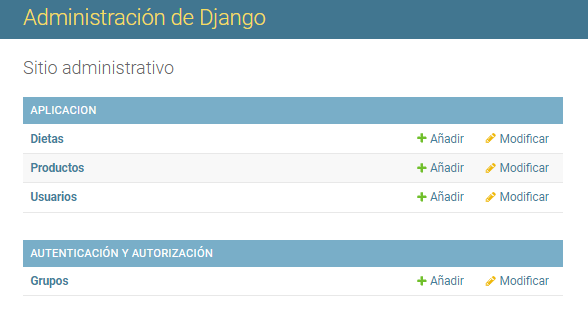
\includegraphics[scale=0.4]{admin.png}}
  \caption{}
\end{figure}

\begin{figure}[H]
  \centering
  \noindent\makebox[\textwidth]{
    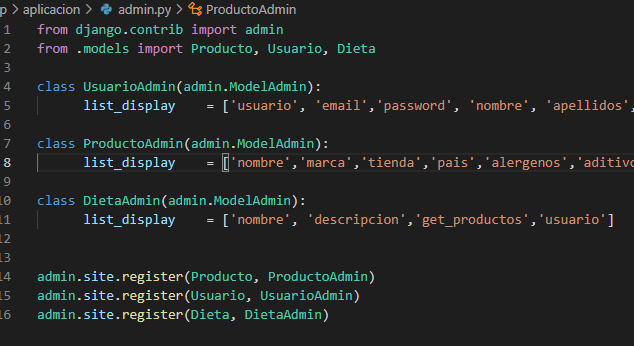
\includegraphics[scale=0.4]{admin.py.png}}
  \caption{}
\end{figure}

\begin{figure}[H]
  \centering
  \noindent\makebox[\textwidth]{
    \includegraphics[scale=0.4]{añadirProducto.png}}
  \caption{}
\end{figure}

\begin{figure}[H]
  \centering
  \noindent\makebox[\textwidth]{
    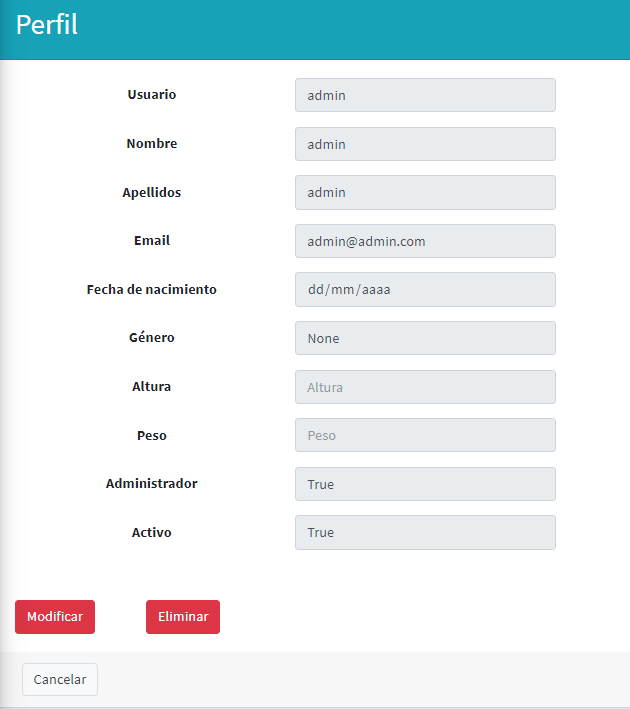
\includegraphics[scale=0.4]{consultarPerfil.png}}
  \caption{}
\end{figure}

\begin{figure}[H]
  \centering
  \noindent\makebox[\textwidth]{
    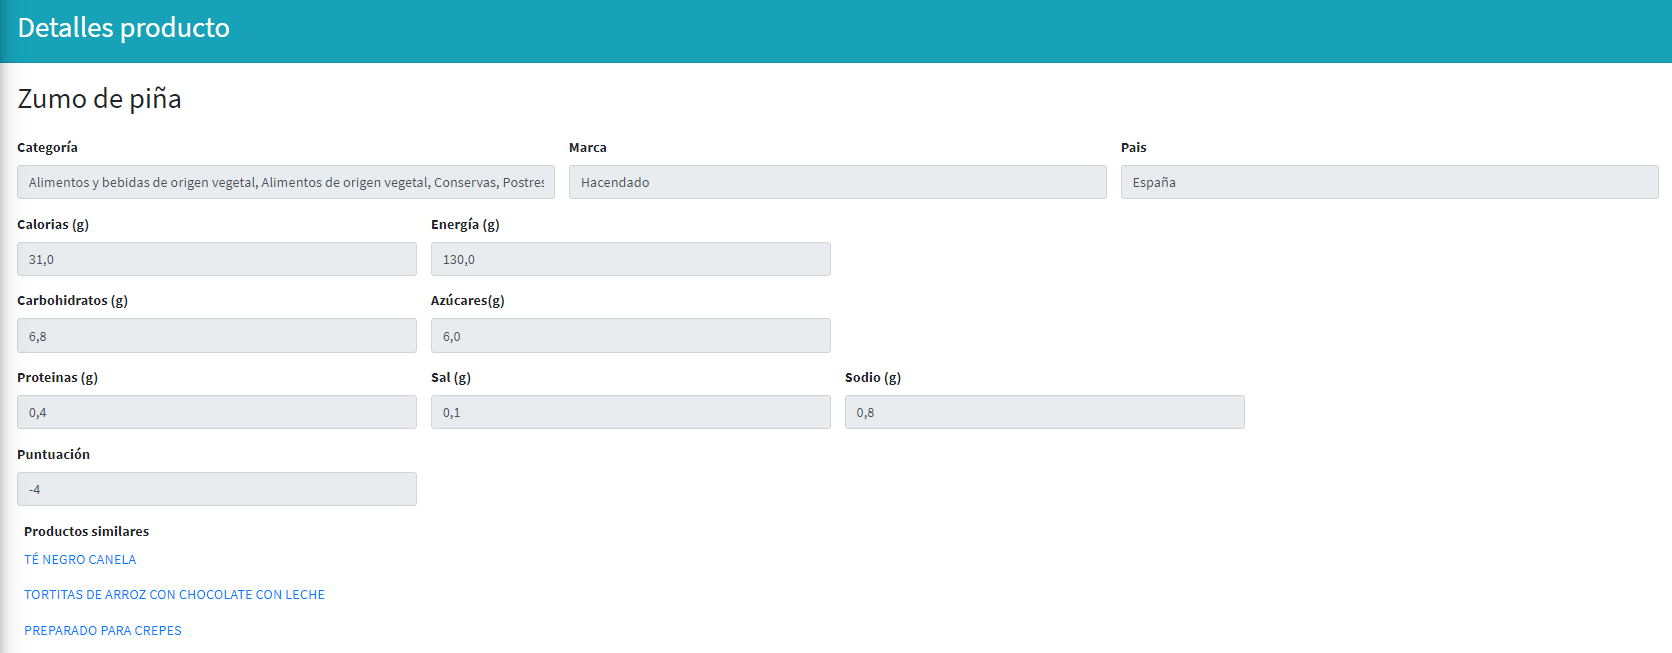
\includegraphics[scale=0.4]{consultarProducto.png}}
  \caption{}
\end{figure}

\begin{figure}[H]
  \centering
  \noindent\makebox[\textwidth]{
    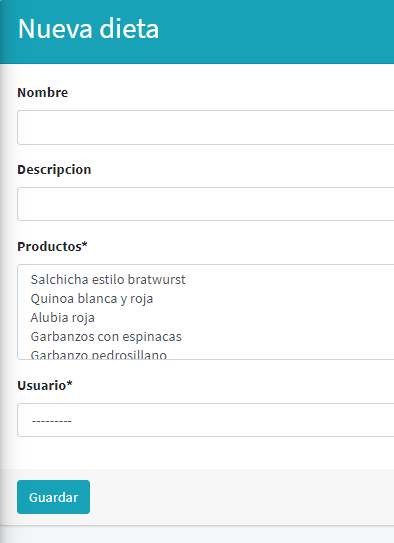
\includegraphics[scale=0.4]{crearDieta.png}}
  \caption{}
\end{figure}

\begin{figure}[H]
  \centering
  \noindent\makebox[\textwidth]{
    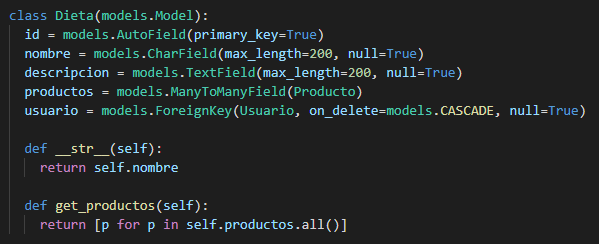
\includegraphics[scale=0.4]{dietaModel.png}}
  \caption{}
\end{figure}

\begin{figure}[H]
  \centering
  \noindent\makebox[\textwidth]{
    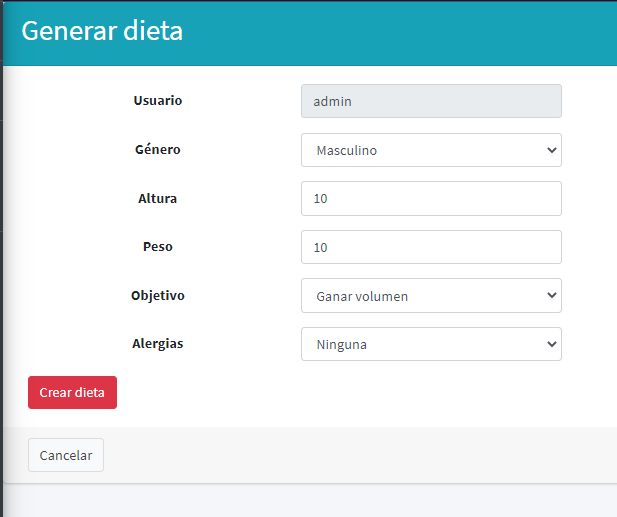
\includegraphics[scale=0.4]{generarDieta.png}}
  \caption{}
\end{figure}

\begin{figure}[H]
  \centering
  \noindent\makebox[\textwidth]{
    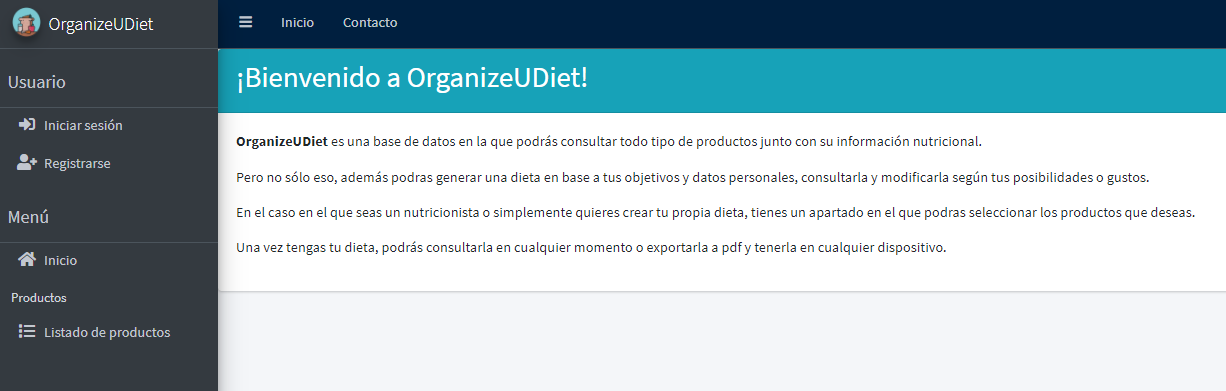
\includegraphics[scale=0.4]{index.png}}
  \caption{}
\end{figure}

\begin{figure}[H]
  \centering
  \noindent\makebox[\textwidth]{
    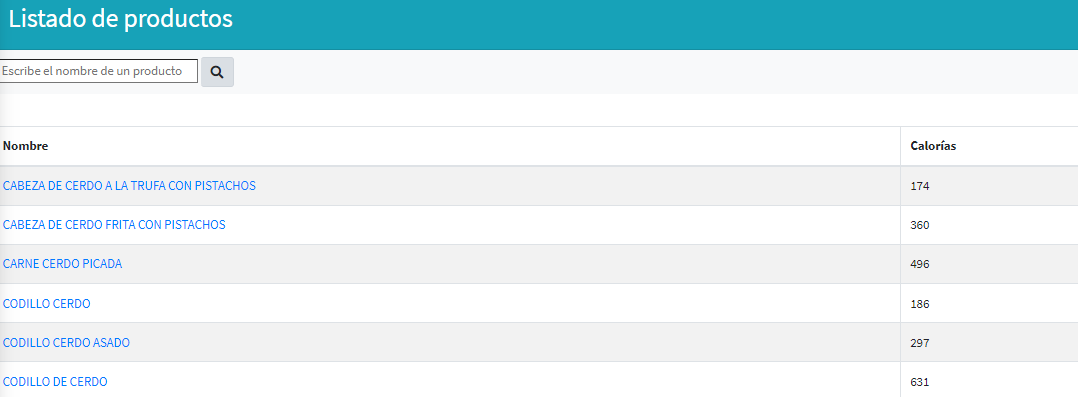
\includegraphics[scale=0.4]{listadoProductos.png}}
  \caption{}
\end{figure}

\begin{figure}[H]
  \centering
  \noindent\makebox[\textwidth]{
    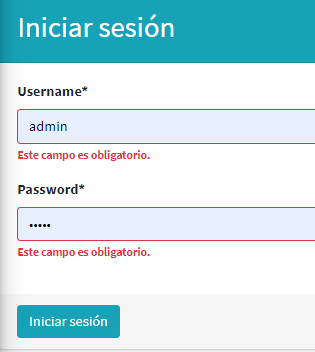
\includegraphics[scale=0.4]{login.png}}
  \caption{}
\end{figure}

\begin{figure}[H]
  \centering
  \noindent\makebox[\textwidth]{
    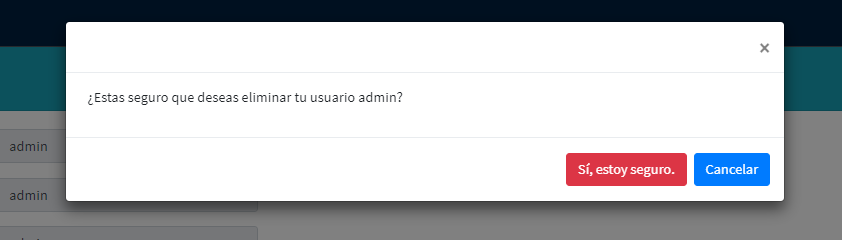
\includegraphics[scale=0.4]{modal.png}}
  \caption{}
\end{figure}

\begin{figure}[H]
  \centering
  \noindent\makebox[\textwidth]{
    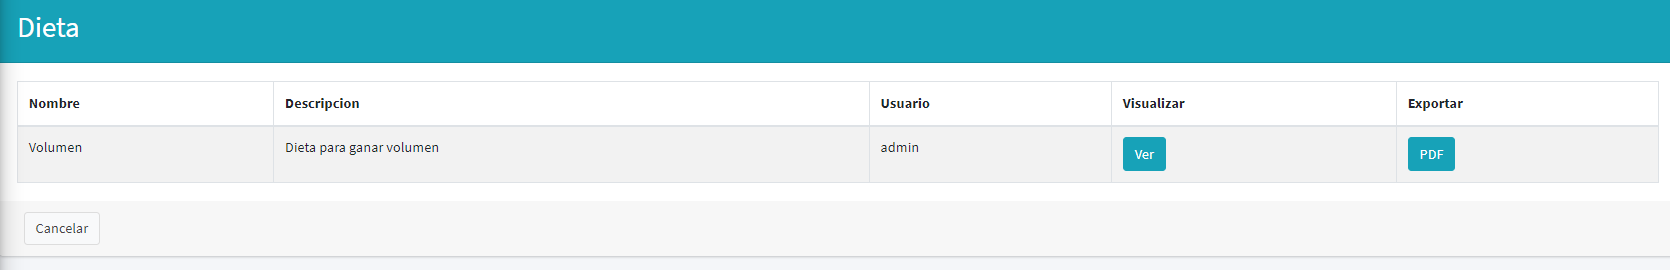
\includegraphics[scale=0.4]{mostrarDieta.png}}
  \caption{}
\end{figure}

\begin{figure}[H]
  \centering
  \noindent\makebox[\textwidth]{
    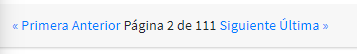
\includegraphics[scale=0.4]{paginador.png}}
  \caption{}
\end{figure}

\begin{figure}[H]
  \centering
  \noindent\makebox[\textwidth]{
    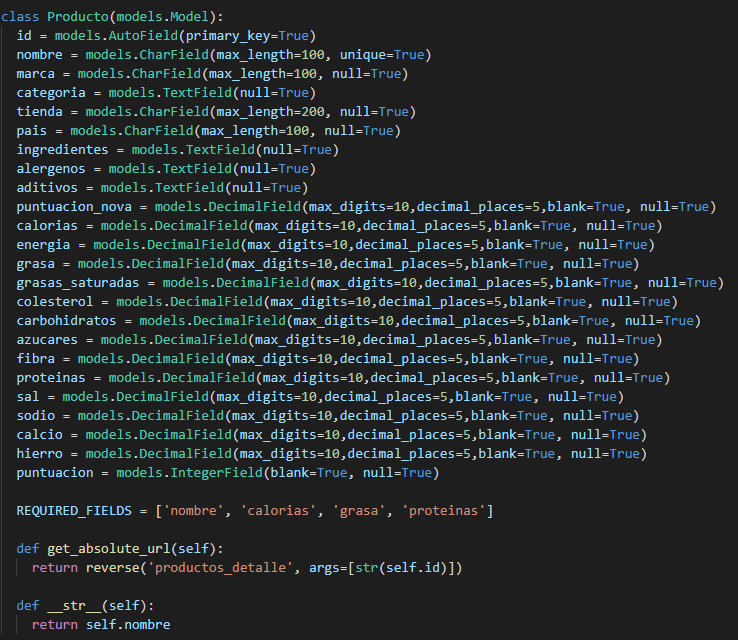
\includegraphics[scale=0.4]{productoModel.png}}
  \caption{}
\end{figure}

\begin{figure}[H]
  \centering
  \noindent\makebox[\textwidth]{
    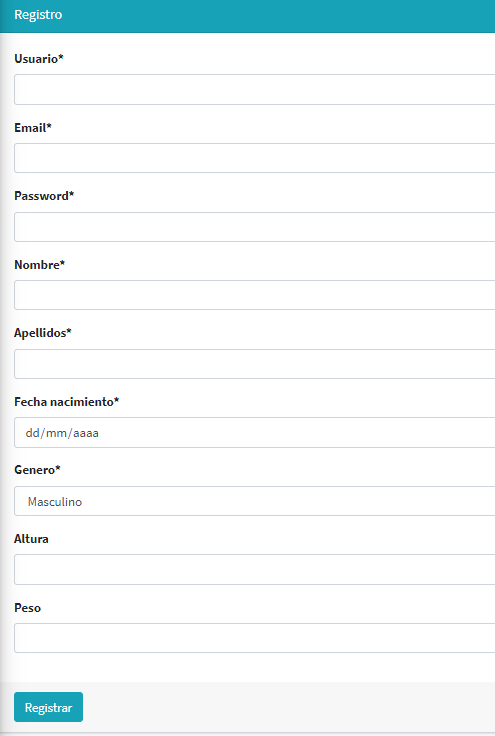
\includegraphics[scale=0.4]{registro.png}}
  \caption{}
\end{figure}

\begin{figure}[H]
  \centering
  \noindent\makebox[\textwidth]{
    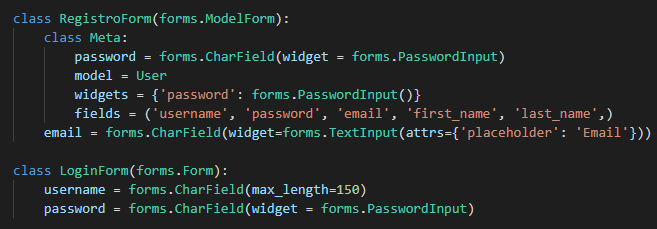
\includegraphics[scale=0.4]{registroLoginForm.png}}
  \caption{}
\end{figure}

\begin{figure}[H]
  \centering
  \noindent\makebox[\textwidth]{
    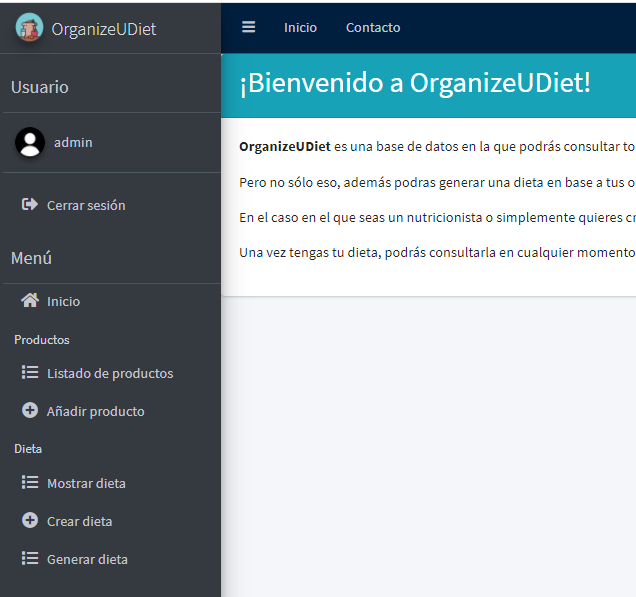
\includegraphics[scale=0.4]{sesionIniciada.png}}
  \caption{}
\end{figure}

\begin{figure}[H]
  \centering
  \noindent\makebox[\textwidth]{
    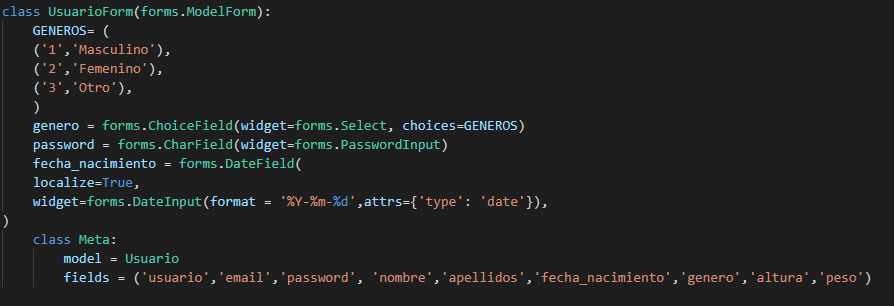
\includegraphics[scale=0.4]{usuarioForm.png}}
  \caption{}
\end{figure}

\begin{figure}[H]
  \centering
  \noindent\makebox[\textwidth]{
    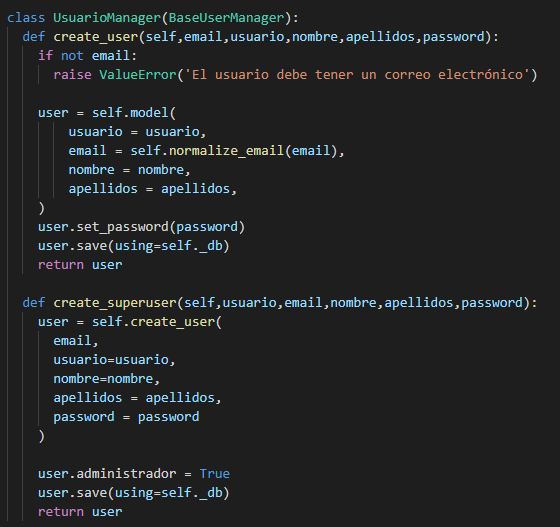
\includegraphics[scale=0.4]{usuarioManager.png}}
  \caption{}
\end{figure}

\begin{figure}[H]
  \centering
  \noindent\makebox[\textwidth]{
    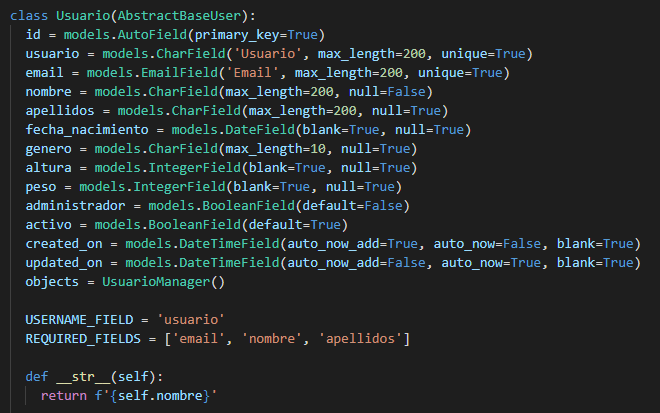
\includegraphics[scale=0.4]{usuarioModel.png}}
  \caption{}
\end{figure}


\section{Tests}

%Librería test - unittest
%Ejemplo

\section{Despliegue}

\subsection{Plataforma}

Por último, quedaría desplegar la aplicación, para ello voy a utilizar \textbf{Heroku}.\\

Ante las necesidades del proyecto de encontrar una plataforma de despliegue en la nube que fuera fácil de usar, pudiera actualizarse de manera automática, fuera gratuita y permitiese el lenguaje Python decidí utilizar Heroku ya que cumplía todas estas necesidades. 

\textbf{Heroku} es una plataforma en la nube que nos permite desplegar aplicaciones web en cualquier lenguaje de programación.
Además es muy sencillo, sólo tenemos que conectar nuestro repositorio de GitHub en el que tengamos el proyecto que queremos desplegar,
podemos configurarlo para que con cada commit se haga el despliegue automaticamente y además es gratuito. Otras alternativas a Heroku 
eran Firebase y Azure.

\subsection{Librerías}

La primera librería que tenemos que instalar es \textbf{Gunicorn}. Esta librería es un servidor HTTP para Unix, sin ella nos sería imposible realizar el despliegue de nuestra aplicación.
Como en este proyecto estamos trabajando con base de datos Postgresql, necesitamos instalar la librería \textbf{psycopg2}. Esta librería es un adaptador a dicha base de datos para el lenguaje Python.\\\\
Heroku por defecto no permite los archivos estáticos, para solucionar este problema he incluido la libreria \textbf{whitenoise}.\\
Esta librería nos permite cargar todos los archivos estáticos y se configura muy fácil, simplemente tenemos que instalarlo y en
el fichero settings.py de la aplicacion incluimos el middleware y las rutas de dichos archivos que queremos cargar.\\\\
Por último, necesitamos dos librerías más, una de ellas es \textbf{dj-database-url}. Esta librería realiza la conexión entre nuestro proyecto y el gestor de base de datos de Heroku.\\
Y la otra librería es \textbf{python-decouple} para usar variables de entorno en Heroku, así evitamos poner tokens y contraseñas a la vista de todos en nuestro proyecto. \\

Por tanto, el archivo requirements.txt quedaría así:
\begin{figure}[H]
  \centering
  \noindent\makebox[\textwidth]{
    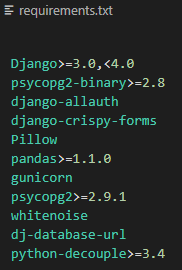
\includegraphics[scale=0.4]{requirements.png}}
  \caption{Archivo requirements.txt}
\end{figure}


\subsection{Configuración}

Para configurar el despliegue en Heroku como he explicado anteriormente debemos registrarnos en la web y conectar el repositorio de Github del proyecto.
Una vez hecho esto nos vamos al archivo settings.py del proyecto y hacemos lo siguiente:\\
Importamos las librerias, ponemos debug a false e incluimos en allowed\_hosts la url de despliegue o simplemente ponemos un asterisco y así acepta todas las urls.

\begin{figure}[H]
  \centering
  \noindent\makebox[\textwidth]{
    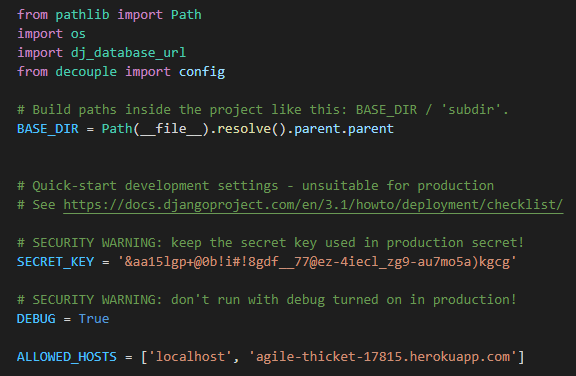
\includegraphics[scale=1]{settings1.png}}
  \caption{Archivo settings.py}
\end{figure}

Añadimos el middleware de whitenoise.

\begin{figure}[H]
  \centering
  \noindent\makebox[\textwidth]{
    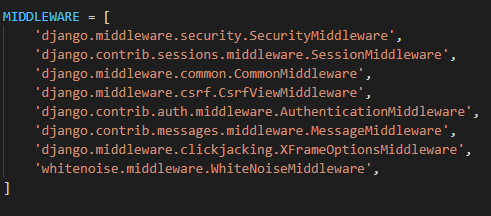
\includegraphics[scale=1]{settings2.png}}
  \caption{Archivo settings.py}
\end{figure}

Indicamos la base de datos.

\begin{figure}[H]
  \centering
  \noindent\makebox[\textwidth]{
    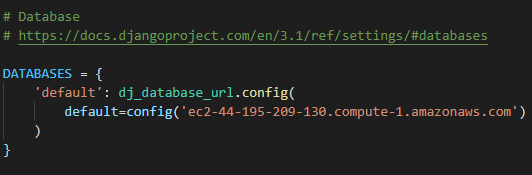
\includegraphics[scale=1]{settings3.png}}
  \caption{Archivo settings.py}
\end{figure}

Añadimos esta línea para que whitenoise cargue los archivos estáticos.

\begin{figure}[H]
  \centering
  \noindent\makebox[\textwidth]{
    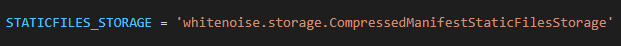
\includegraphics[scale=1]{settings4.png}}
  \caption{Archivo settings.py}
\end{figure}

Ya tendriamos configurado todo. Simplemente tenemos que esperar a que se haga el despliegue si hemos configurado que se haga automaticamente con cada commit o desplegarlo nosotros desde la web.\\\\

Otra opción sería hacerlo desde local.
Nos conectamos a nuestra cuenta de Heroku con heroku login, creamos una app de heroku con heroku create y hacemos un push desde nuestro repositorio local con:
\begin{lstlisting}
git push --prefix app keroku master
\end{lstlisting}

Conectamos nuestra base de datos con nuestra app con el siguiente comando:
\begin{lstlisting}
heroku pg:psql <nombre_bd_heroku> --app <nombre_app_heroku>
\end{lstlisting}

Ahora sólo quedaría hacer un migrate de la base de datos con:
\begin{lstlisting}
heroku run python manage.py migrate
\end{lstlisting}

Incluimos nuestros archivos sql con nuestros datos de la base de datos.
\begin{lstlisting}
heroku pg:psql --app <nombre_app> < <archivo.sql>
\end{lstlisting}
Y abrimos la aplicación con heroku open.\\\\

Para probar la aplicación aquí dejo el enlace:

\url{https://agile-thicket-17815.herokuapp.com/}